%\documentclass{standalone}
%\usepackage{tikz}
%\usetikzlibrary{patterns,plotmarks}
%\begin{document}
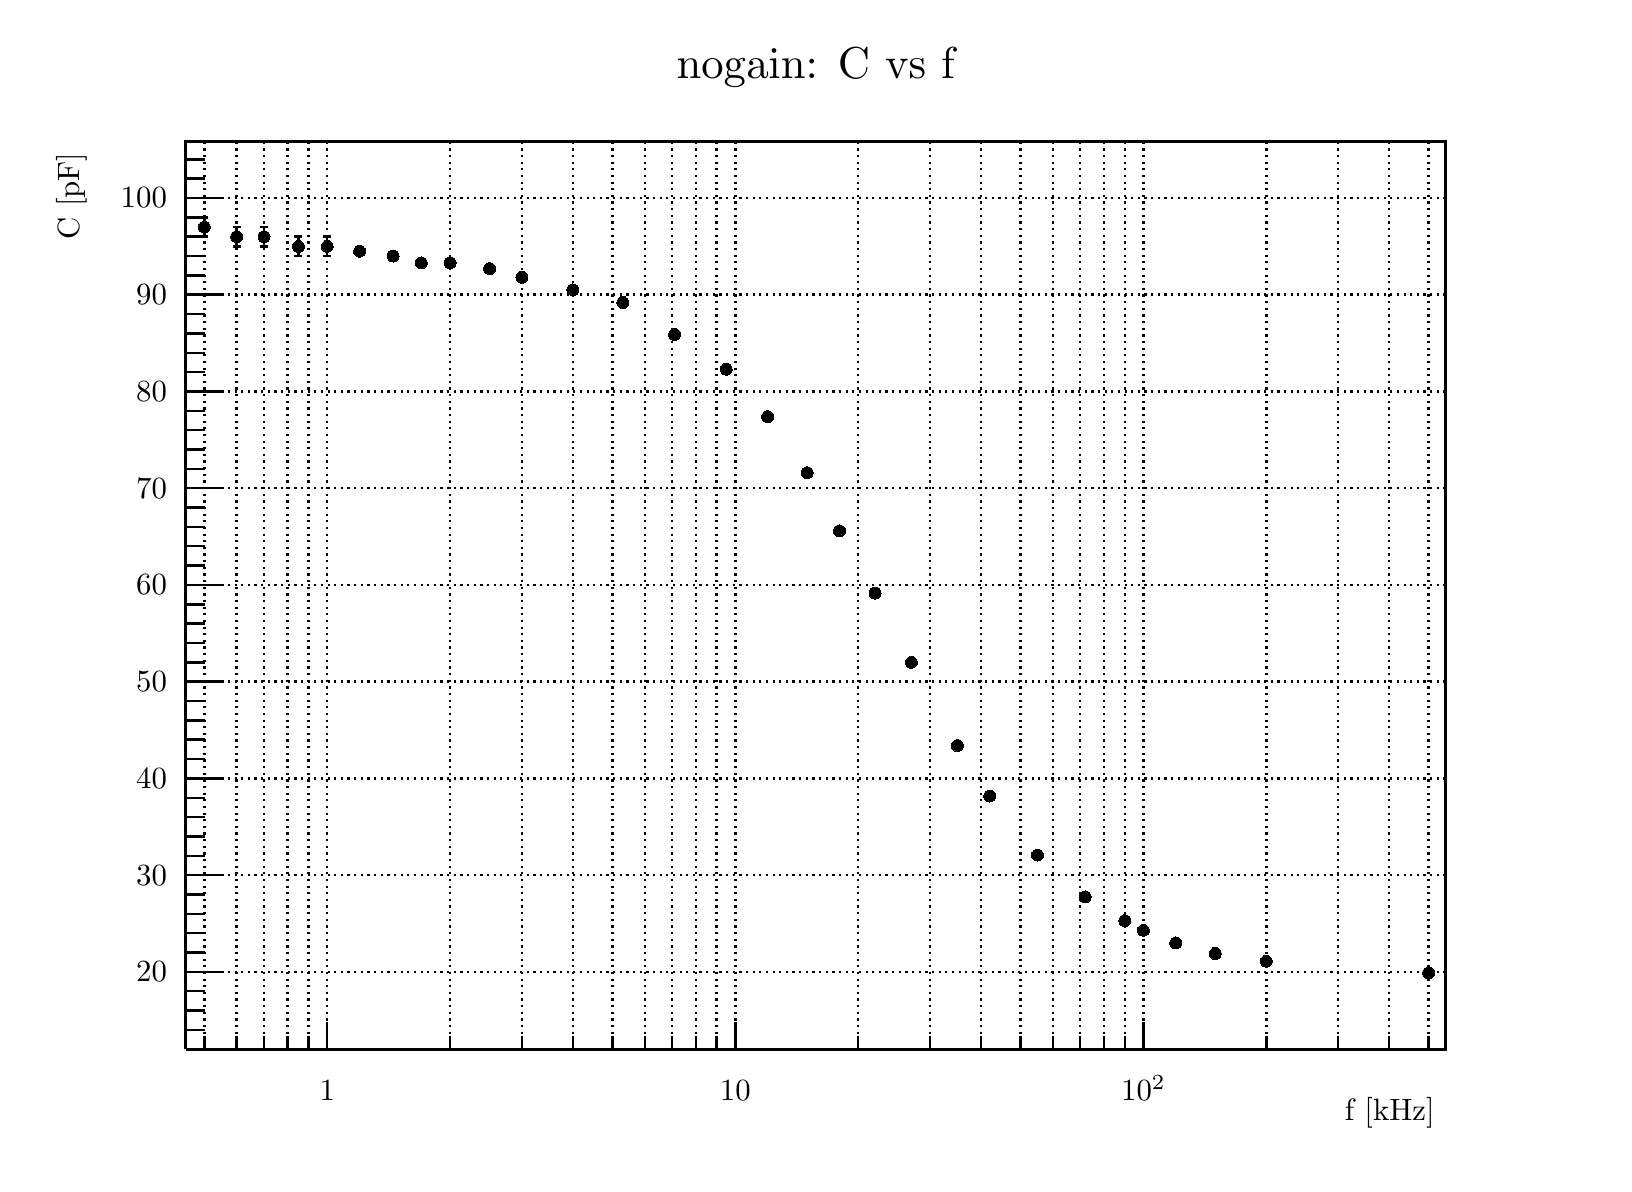
\begin{tikzpicture}
\def\CheckTikzLibraryLoaded#1{ \ifcsname tikz@library@#1@loaded\endcsname \else \PackageWarning{tikz}{usetikzlibrary{#1} is missing in the preamble.} \fi }
\CheckTikzLibraryLoaded{patterns}
\CheckTikzLibraryLoaded{plotmarks}
\pgfdeclareplotmark{cross} {
\pgfpathmoveto{\pgfpoint{-0.3\pgfplotmarksize}{\pgfplotmarksize}}
\pgfpathlineto{\pgfpoint{+0.3\pgfplotmarksize}{\pgfplotmarksize}}
\pgfpathlineto{\pgfpoint{+0.3\pgfplotmarksize}{0.3\pgfplotmarksize}}
\pgfpathlineto{\pgfpoint{+1\pgfplotmarksize}{0.3\pgfplotmarksize}}
\pgfpathlineto{\pgfpoint{+1\pgfplotmarksize}{-0.3\pgfplotmarksize}}
\pgfpathlineto{\pgfpoint{+0.3\pgfplotmarksize}{-0.3\pgfplotmarksize}}
\pgfpathlineto{\pgfpoint{+0.3\pgfplotmarksize}{-1.\pgfplotmarksize}}
\pgfpathlineto{\pgfpoint{-0.3\pgfplotmarksize}{-1.\pgfplotmarksize}}
\pgfpathlineto{\pgfpoint{-0.3\pgfplotmarksize}{-0.3\pgfplotmarksize}}
\pgfpathlineto{\pgfpoint{-1.\pgfplotmarksize}{-0.3\pgfplotmarksize}}
\pgfpathlineto{\pgfpoint{-1.\pgfplotmarksize}{0.3\pgfplotmarksize}}
\pgfpathlineto{\pgfpoint{-0.3\pgfplotmarksize}{0.3\pgfplotmarksize}}
\pgfpathclose
\pgfusepathqstroke
}
\pgfdeclareplotmark{cross*} {
\pgfpathmoveto{\pgfpoint{-0.3\pgfplotmarksize}{\pgfplotmarksize}}
\pgfpathlineto{\pgfpoint{+0.3\pgfplotmarksize}{\pgfplotmarksize}}
\pgfpathlineto{\pgfpoint{+0.3\pgfplotmarksize}{0.3\pgfplotmarksize}}
\pgfpathlineto{\pgfpoint{+1\pgfplotmarksize}{0.3\pgfplotmarksize}}
\pgfpathlineto{\pgfpoint{+1\pgfplotmarksize}{-0.3\pgfplotmarksize}}
\pgfpathlineto{\pgfpoint{+0.3\pgfplotmarksize}{-0.3\pgfplotmarksize}}
\pgfpathlineto{\pgfpoint{+0.3\pgfplotmarksize}{-1.\pgfplotmarksize}}
\pgfpathlineto{\pgfpoint{-0.3\pgfplotmarksize}{-1.\pgfplotmarksize}}
\pgfpathlineto{\pgfpoint{-0.3\pgfplotmarksize}{-0.3\pgfplotmarksize}}
\pgfpathlineto{\pgfpoint{-1.\pgfplotmarksize}{-0.3\pgfplotmarksize}}
\pgfpathlineto{\pgfpoint{-1.\pgfplotmarksize}{0.3\pgfplotmarksize}}
\pgfpathlineto{\pgfpoint{-0.3\pgfplotmarksize}{0.3\pgfplotmarksize}}
\pgfpathclose
\pgfusepathqfillstroke
}
\pgfdeclareplotmark{newstar} {
\pgfpathmoveto{\pgfqpoint{0pt}{\pgfplotmarksize}}
\pgfpathlineto{\pgfqpointpolar{44}{0.5\pgfplotmarksize}}
\pgfpathlineto{\pgfqpointpolar{18}{\pgfplotmarksize}}
\pgfpathlineto{\pgfqpointpolar{-20}{0.5\pgfplotmarksize}}
\pgfpathlineto{\pgfqpointpolar{-54}{\pgfplotmarksize}}
\pgfpathlineto{\pgfqpointpolar{-90}{0.5\pgfplotmarksize}}
\pgfpathlineto{\pgfqpointpolar{234}{\pgfplotmarksize}}
\pgfpathlineto{\pgfqpointpolar{198}{0.5\pgfplotmarksize}}
\pgfpathlineto{\pgfqpointpolar{162}{\pgfplotmarksize}}
\pgfpathlineto{\pgfqpointpolar{134}{0.5\pgfplotmarksize}}
\pgfpathclose
\pgfusepathqstroke
}
\pgfdeclareplotmark{newstar*} {
\pgfpathmoveto{\pgfqpoint{0pt}{\pgfplotmarksize}}
\pgfpathlineto{\pgfqpointpolar{44}{0.5\pgfplotmarksize}}
\pgfpathlineto{\pgfqpointpolar{18}{\pgfplotmarksize}}
\pgfpathlineto{\pgfqpointpolar{-20}{0.5\pgfplotmarksize}}
\pgfpathlineto{\pgfqpointpolar{-54}{\pgfplotmarksize}}
\pgfpathlineto{\pgfqpointpolar{-90}{0.5\pgfplotmarksize}}
\pgfpathlineto{\pgfqpointpolar{234}{\pgfplotmarksize}}
\pgfpathlineto{\pgfqpointpolar{198}{0.5\pgfplotmarksize}}
\pgfpathlineto{\pgfqpointpolar{162}{\pgfplotmarksize}}
\pgfpathlineto{\pgfqpointpolar{134}{0.5\pgfplotmarksize}}
\pgfpathclose
\pgfusepathqfillstroke
}
\definecolor{c}{rgb}{1,1,1};
\draw [color=c, fill=c] (0,0) rectangle (20,14.411);
\draw [color=c, fill=c] (2,1.4411) rectangle (18,12.9699);
\definecolor{c}{rgb}{0,0,0};
\draw [c,line width=0.9] (2,1.4411) -- (2,12.9699) -- (18,12.9699) -- (18,1.4411) -- (2,1.4411);
\definecolor{c}{rgb}{1,1,1};
\draw [color=c, fill=c] (2,1.4411) rectangle (18,12.9699);
\definecolor{c}{rgb}{0,0,0};
\draw [c,line width=0.9] (2,1.4411) -- (2,12.9699) -- (18,12.9699) -- (18,1.4411) -- (2,1.4411);
\draw [c,line width=0.9] (2,1.4411) -- (18,1.4411);
\draw [c,dash pattern=on 0.80pt off 1.60pt ,line width=0.9] (2.23716,12.9699) -- (2.23716,1.4411);
\draw [c,dash pattern=on 0.80pt off 1.60pt ,line width=0.9] (2.64754,12.9699) -- (2.64754,1.4411);
\draw [c,dash pattern=on 0.80pt off 1.60pt ,line width=0.9] (2.99452,12.9699) -- (2.99452,1.4411);
\draw [c,dash pattern=on 0.80pt off 1.60pt ,line width=0.9] (3.29508,12.9699) -- (3.29508,1.4411);
\draw [c,dash pattern=on 0.80pt off 1.60pt ,line width=0.9] (3.56019,12.9699) -- (3.56019,1.4411);
\draw [c,dash pattern=on 0.80pt off 1.60pt ,line width=0.9] (3.79735,12.9699) -- (3.79735,1.4411);
\draw [c,dash pattern=on 0.80pt off 1.60pt ,line width=0.9] (5.35754,12.9699) -- (5.35754,1.4411);
\draw [c,dash pattern=on 0.80pt off 1.60pt ,line width=0.9] (6.27019,12.9699) -- (6.27019,1.4411);
\draw [c,dash pattern=on 0.80pt off 1.60pt ,line width=0.9] (6.91773,12.9699) -- (6.91773,1.4411);
\draw [c,dash pattern=on 0.80pt off 1.60pt ,line width=0.9] (7.42,12.9699) -- (7.42,1.4411);
\draw [c,dash pattern=on 0.80pt off 1.60pt ,line width=0.9] (7.83038,12.9699) -- (7.83038,1.4411);
\draw [c,dash pattern=on 0.80pt off 1.60pt ,line width=0.9] (8.17735,12.9699) -- (8.17735,1.4411);
\draw [c,dash pattern=on 0.80pt off 1.60pt ,line width=0.9] (8.47792,12.9699) -- (8.47792,1.4411);
\draw [c,dash pattern=on 0.80pt off 1.60pt ,line width=0.9] (8.74303,12.9699) -- (8.74303,1.4411);
\draw [c,dash pattern=on 0.80pt off 1.60pt ,line width=0.9] (8.98019,12.9699) -- (8.98019,1.4411);
\draw [c,dash pattern=on 0.80pt off 1.60pt ,line width=0.9] (10.5404,12.9699) -- (10.5404,1.4411);
\draw [c,dash pattern=on 0.80pt off 1.60pt ,line width=0.9] (11.453,12.9699) -- (11.453,1.4411);
\draw [c,dash pattern=on 0.80pt off 1.60pt ,line width=0.9] (12.1006,12.9699) -- (12.1006,1.4411);
\draw [c,dash pattern=on 0.80pt off 1.60pt ,line width=0.9] (12.6028,12.9699) -- (12.6028,1.4411);
\draw [c,dash pattern=on 0.80pt off 1.60pt ,line width=0.9] (13.0132,12.9699) -- (13.0132,1.4411);
\draw [c,dash pattern=on 0.80pt off 1.60pt ,line width=0.9] (13.3602,12.9699) -- (13.3602,1.4411);
\draw [c,dash pattern=on 0.80pt off 1.60pt ,line width=0.9] (13.6608,12.9699) -- (13.6608,1.4411);
\draw [c,dash pattern=on 0.80pt off 1.60pt ,line width=0.9] (13.9259,12.9699) -- (13.9259,1.4411);
\draw [c,dash pattern=on 0.80pt off 1.60pt ,line width=0.9] (14.163,12.9699) -- (14.163,1.4411);
\draw [c,dash pattern=on 0.80pt off 1.60pt ,line width=0.9] (15.7232,12.9699) -- (15.7232,1.4411);
\draw [c,dash pattern=on 0.80pt off 1.60pt ,line width=0.9] (16.6359,12.9699) -- (16.6359,1.4411);
\draw [c,dash pattern=on 0.80pt off 1.60pt ,line width=0.9] (17.2834,12.9699) -- (17.2834,1.4411);
\draw [c,dash pattern=on 0.80pt off 1.60pt ,line width=0.9] (17.7857,12.9699) -- (17.7857,1.4411);
\draw [c,line width=0.9] (2,1.4411) -- (2,12.9699);
\draw [c,dash pattern=on 0.80pt off 1.60pt ,line width=0.9] (18,2.42641) -- (2,2.42641);
\draw [c,dash pattern=on 0.80pt off 1.60pt ,line width=0.9] (18,3.65497) -- (2,3.65497);
\draw [c,dash pattern=on 0.80pt off 1.60pt ,line width=0.9] (18,4.88353) -- (2,4.88353);
\draw [c,dash pattern=on 0.80pt off 1.60pt ,line width=0.9] (18,6.11209) -- (2,6.11209);
\draw [c,dash pattern=on 0.80pt off 1.60pt ,line width=0.9] (18,7.34066) -- (2,7.34066);
\draw [c,dash pattern=on 0.80pt off 1.60pt ,line width=0.9] (18,8.56922) -- (2,8.56922);
\draw [c,dash pattern=on 0.80pt off 1.60pt ,line width=0.9] (18,9.79778) -- (2,9.79778);
\draw [c,dash pattern=on 0.80pt off 1.60pt ,line width=0.9] (18,11.0263) -- (2,11.0263);
\draw [c,dash pattern=on 0.80pt off 1.60pt ,line width=0.9] (18,12.2549) -- (2,12.2549);
\draw [c,dash pattern=on 0.80pt off 1.60pt ,line width=0.9] (18,2.42641) -- (2,2.42641);
\draw [c,dash pattern=on 0.80pt off 1.60pt ,line width=0.9] (18,12.2549) -- (2,12.2549);
\draw [c,line width=0.9] (2,1.4411) -- (18,1.4411);
\draw [c,line width=0.9] (2.23716,1.61404) -- (2.23716,1.4411);
\draw [c,line width=0.9] (2.64754,1.61404) -- (2.64754,1.4411);
\draw [c,line width=0.9] (2.99452,1.61404) -- (2.99452,1.4411);
\draw [c,line width=0.9] (3.29508,1.61404) -- (3.29508,1.4411);
\draw [c,line width=0.9] (3.56019,1.61404) -- (3.56019,1.4411);
\draw [c,line width=0.9] (3.79735,1.78697) -- (3.79735,1.4411);
\draw [anchor=base] (3.79735,0.789004) node[scale=1.11327, color=c, rotate=0]{1};
\draw [c,line width=0.9] (5.35754,1.61404) -- (5.35754,1.4411);
\draw [c,line width=0.9] (6.27019,1.61404) -- (6.27019,1.4411);
\draw [c,line width=0.9] (6.91773,1.61404) -- (6.91773,1.4411);
\draw [c,line width=0.9] (7.42,1.61404) -- (7.42,1.4411);
\draw [c,line width=0.9] (7.83038,1.61404) -- (7.83038,1.4411);
\draw [c,line width=0.9] (8.17735,1.61404) -- (8.17735,1.4411);
\draw [c,line width=0.9] (8.47792,1.61404) -- (8.47792,1.4411);
\draw [c,line width=0.9] (8.74303,1.61404) -- (8.74303,1.4411);
\draw [c,line width=0.9] (8.98019,1.78697) -- (8.98019,1.4411);
\draw [anchor=base] (8.98019,0.789004) node[scale=1.11327, color=c, rotate=0]{10};
\draw [c,line width=0.9] (10.5404,1.61404) -- (10.5404,1.4411);
\draw [c,line width=0.9] (11.453,1.61404) -- (11.453,1.4411);
\draw [c,line width=0.9] (12.1006,1.61404) -- (12.1006,1.4411);
\draw [c,line width=0.9] (12.6028,1.61404) -- (12.6028,1.4411);
\draw [c,line width=0.9] (13.0132,1.61404) -- (13.0132,1.4411);
\draw [c,line width=0.9] (13.3602,1.61404) -- (13.3602,1.4411);
\draw [c,line width=0.9] (13.6608,1.61404) -- (13.6608,1.4411);
\draw [c,line width=0.9] (13.9259,1.61404) -- (13.9259,1.4411);
\draw [c,line width=0.9] (14.163,1.78697) -- (14.163,1.4411);
\draw [anchor=base] (14.163,0.789004) node[scale=1.11327, color=c, rotate=0]{$10^{2}$};
\draw [c,line width=0.9] (15.7232,1.61404) -- (15.7232,1.4411);
\draw [c,line width=0.9] (16.6359,1.61404) -- (16.6359,1.4411);
\draw [c,line width=0.9] (17.2834,1.61404) -- (17.2834,1.4411);
\draw [c,line width=0.9] (17.7857,1.61404) -- (17.7857,1.4411);
\draw [anchor= east] (18,0.634085) node[scale=1.11327, color=c, rotate=0]{f [kHz]};
\draw [c,line width=0.9] (2,1.4411) -- (2,12.9699);
\draw [c,line width=0.9] (2.48,2.42641) -- (2,2.42641);
\draw [c,line width=0.9] (2.24,2.67212) -- (2,2.67212);
\draw [c,line width=0.9] (2.24,2.91783) -- (2,2.91783);
\draw [c,line width=0.9] (2.24,3.16355) -- (2,3.16355);
\draw [c,line width=0.9] (2.24,3.40926) -- (2,3.40926);
\draw [c,line width=0.9] (2.48,3.65497) -- (2,3.65497);
\draw [c,line width=0.9] (2.24,3.90068) -- (2,3.90068);
\draw [c,line width=0.9] (2.24,4.1464) -- (2,4.1464);
\draw [c,line width=0.9] (2.24,4.39211) -- (2,4.39211);
\draw [c,line width=0.9] (2.24,4.63782) -- (2,4.63782);
\draw [c,line width=0.9] (2.48,4.88353) -- (2,4.88353);
\draw [c,line width=0.9] (2.24,5.12924) -- (2,5.12924);
\draw [c,line width=0.9] (2.24,5.37496) -- (2,5.37496);
\draw [c,line width=0.9] (2.24,5.62067) -- (2,5.62067);
\draw [c,line width=0.9] (2.24,5.86638) -- (2,5.86638);
\draw [c,line width=0.9] (2.48,6.11209) -- (2,6.11209);
\draw [c,line width=0.9] (2.24,6.35781) -- (2,6.35781);
\draw [c,line width=0.9] (2.24,6.60352) -- (2,6.60352);
\draw [c,line width=0.9] (2.24,6.84923) -- (2,6.84923);
\draw [c,line width=0.9] (2.24,7.09494) -- (2,7.09494);
\draw [c,line width=0.9] (2.48,7.34066) -- (2,7.34066);
\draw [c,line width=0.9] (2.24,7.58637) -- (2,7.58637);
\draw [c,line width=0.9] (2.24,7.83208) -- (2,7.83208);
\draw [c,line width=0.9] (2.24,8.07779) -- (2,8.07779);
\draw [c,line width=0.9] (2.24,8.32351) -- (2,8.32351);
\draw [c,line width=0.9] (2.48,8.56922) -- (2,8.56922);
\draw [c,line width=0.9] (2.24,8.81493) -- (2,8.81493);
\draw [c,line width=0.9] (2.24,9.06064) -- (2,9.06064);
\draw [c,line width=0.9] (2.24,9.30635) -- (2,9.30635);
\draw [c,line width=0.9] (2.24,9.55207) -- (2,9.55207);
\draw [c,line width=0.9] (2.48,9.79778) -- (2,9.79778);
\draw [c,line width=0.9] (2.24,10.0435) -- (2,10.0435);
\draw [c,line width=0.9] (2.24,10.2892) -- (2,10.2892);
\draw [c,line width=0.9] (2.24,10.5349) -- (2,10.5349);
\draw [c,line width=0.9] (2.24,10.7806) -- (2,10.7806);
\draw [c,line width=0.9] (2.48,11.0263) -- (2,11.0263);
\draw [c,line width=0.9] (2.24,11.2721) -- (2,11.2721);
\draw [c,line width=0.9] (2.24,11.5178) -- (2,11.5178);
\draw [c,line width=0.9] (2.24,11.7635) -- (2,11.7635);
\draw [c,line width=0.9] (2.24,12.0092) -- (2,12.0092);
\draw [c,line width=0.9] (2.48,12.2549) -- (2,12.2549);
\draw [c,line width=0.9] (2.48,2.42641) -- (2,2.42641);
\draw [c,line width=0.9] (2.24,2.1807) -- (2,2.1807);
\draw [c,line width=0.9] (2.24,1.93498) -- (2,1.93498);
\draw [c,line width=0.9] (2.24,1.68927) -- (2,1.68927);
\draw [c,line width=0.9] (2.24,1.44356) -- (2,1.44356);
\draw [c,line width=0.9] (2.48,12.2549) -- (2,12.2549);
\draw [c,line width=0.9] (2.24,12.5006) -- (2,12.5006);
\draw [c,line width=0.9] (2.24,12.7463) -- (2,12.7463);
\draw [anchor= east] (1.9,2.42641) node[scale=1.11327, color=c, rotate=0]{20};
\draw [anchor= east] (1.9,3.65497) node[scale=1.11327, color=c, rotate=0]{30};
\draw [anchor= east] (1.9,4.88353) node[scale=1.11327, color=c, rotate=0]{40};
\draw [anchor= east] (1.9,6.11209) node[scale=1.11327, color=c, rotate=0]{50};
\draw [anchor= east] (1.9,7.34066) node[scale=1.11327, color=c, rotate=0]{60};
\draw [anchor= east] (1.9,8.56922) node[scale=1.11327, color=c, rotate=0]{70};
\draw [anchor= east] (1.9,9.79778) node[scale=1.11327, color=c, rotate=0]{80};
\draw [anchor= east] (1.9,11.0263) node[scale=1.11327, color=c, rotate=0]{90};
\draw [anchor= east] (1.9,12.2549) node[scale=1.11327, color=c, rotate=0]{100};
\draw [anchor= east] (0.54812,12.9699) node[scale=1.11327, color=c, rotate=90]{C [pF]};
\foreach \P in {(2.23715,11.8863), (2.64754,11.7635), (2.99451,11.7635), (3.43153,11.6406), (3.79734,11.6406), (4.20773,11.5792), (4.63369,11.5178), (4.99172,11.4318), (5.35753,11.4318), (5.8598,11.3581), (6.27019,11.2475), (6.91772,11.0878),
 (7.55115,10.9281), (8.20928,10.5226), (8.86473,10.0803), (9.39057,9.47835), (9.89284,8.76579), (10.3032,8.02865), (10.7549,7.23623), (11.2159,6.35781), (11.8,5.30124), (12.2104,4.65993), (12.8174,3.91051), (13.4236,3.37977), (13.9259,3.07755),
 (14.163,2.95469), (14.5734,2.79498), (15.0757,2.65984), (15.7232,2.56155), (17.7857,2.41412)}{\draw[mark options={color=c,fill=c},mark size=2.162162pt, line width=0.000000pt, mark=*] plot coordinates {\P};}
\draw [c,line width=0.9] (2.23715,11.9615) -- (2.23715,12.0092);
\draw [c,line width=0.9] (2.23715,11.8111) -- (2.23715,11.7635);
\draw [c,line width=0.9] (2.18703,12.0092) -- (2.28728,12.0092);
\draw [c,line width=0.9] (2.18703,11.7635) -- (2.28728,11.7635);
\draw [c,line width=0.9] (2.64754,11.8387) -- (2.64754,11.8863);
\draw [c,line width=0.9] (2.64754,11.6883) -- (2.64754,11.6406);
\draw [c,line width=0.9] (2.59741,11.8863) -- (2.69766,11.8863);
\draw [c,line width=0.9] (2.59741,11.6406) -- (2.69766,11.6406);
\draw [c,line width=0.9] (2.99451,11.8387) -- (2.99451,11.8863);
\draw [c,line width=0.9] (2.99451,11.6883) -- (2.99451,11.6406);
\draw [c,line width=0.9] (2.94439,11.8863) -- (3.04464,11.8863);
\draw [c,line width=0.9] (2.94439,11.6406) -- (3.04464,11.6406);
\draw [c,line width=0.9] (3.43153,11.7158) -- (3.43153,11.7635);
\draw [c,line width=0.9] (3.43153,11.5654) -- (3.43153,11.5178);
\draw [c,line width=0.9] (3.38141,11.7635) -- (3.48166,11.7635);
\draw [c,line width=0.9] (3.38141,11.5178) -- (3.48166,11.5178);
\draw [c,line width=0.9] (3.79734,11.7158) -- (3.79734,11.7635);
\draw [c,line width=0.9] (3.79734,11.5654) -- (3.79734,11.5178);
\draw [c,line width=0.9] (3.74722,11.7635) -- (3.84747,11.7635);
\draw [c,line width=0.9] (3.74722,11.5178) -- (3.84747,11.5178);
\draw (10,13.9179) node[scale=1.61424, color=c, rotate=0]{nogain: C vs f};
\end{tikzpicture}
%\end{document}
